\documentclass{minimal}
\usepackage{tikz}
\usetikzlibrary{shadows.blur}
\def\C{circle [radius=.4]}
\begin{document}
\newpage
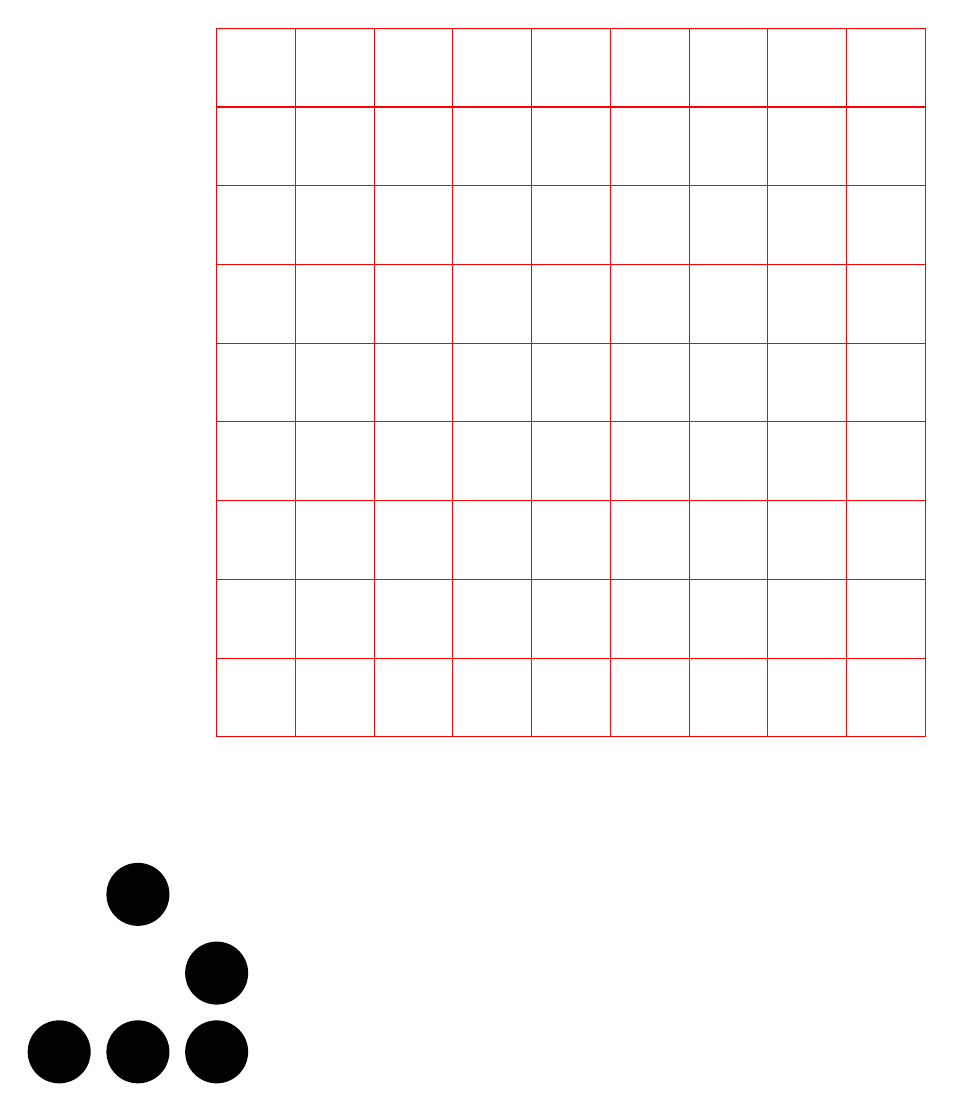
\begin{tikzpicture}
\draw [color=red,xshift=3cm,yshift=5cm] (0,0) grid (9,9);
\fill
(1,1) \C
(2,1) \C
(2,3) \C
(3,2) \C
(3,1) \C;
\end{tikzpicture}
\newpage
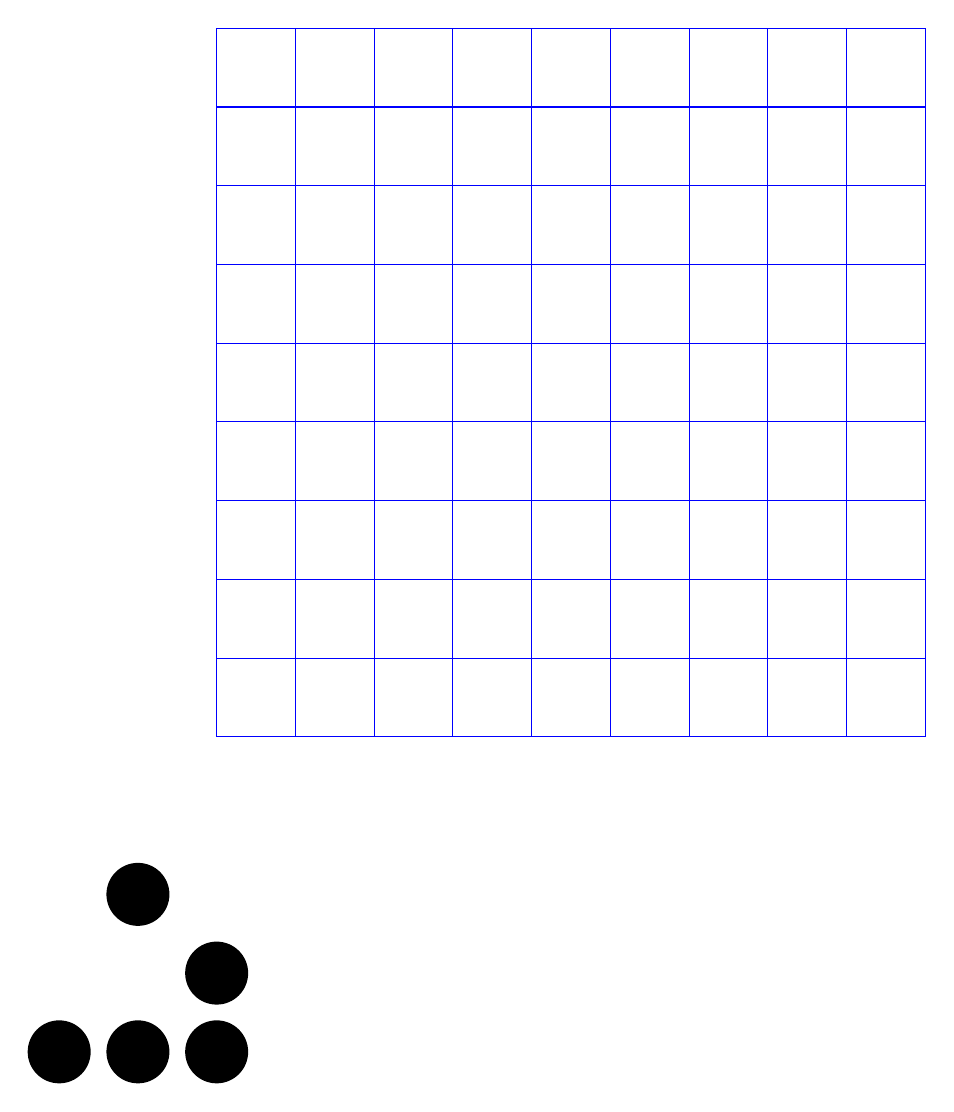
\begin{tikzpicture}
\draw [color=blue,xshift=3cm,yshift=5cm] (0,0) grid (9,9);
\fill
(1,1) \C
(2,1) \C
(2,3) \C
(3,2) \C
(3,1) \C;
\end{tikzpicture}
\newpage
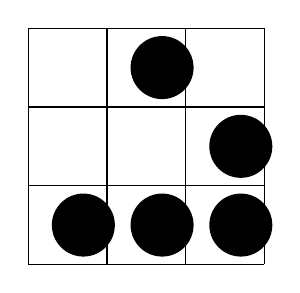
\begin{tikzpicture}
\draw [xshift=0.3cm,yshift=.5cm] (0,0) grid (3,3);
\fill
(1,1) \C
(2,1) \C
(2,3) \C
(3,2) \C
(3,1) \C;
\end{tikzpicture}
\newpage
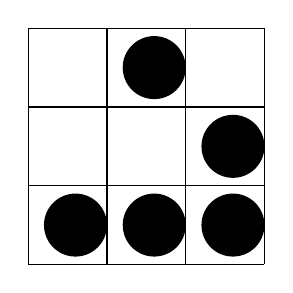
\begin{tikzpicture}
\draw [xshift=0.4cm,yshift=.5cm] (0,0) grid (3,3);
\fill
(1,1) \C
(2,1) \C
(2,3) \C
(3,2) \C
(3,1) \C;
\end{tikzpicture}
\newpage
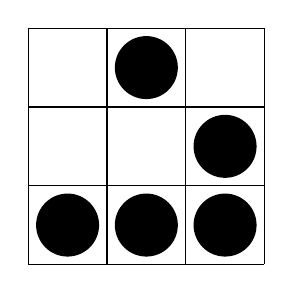
\begin{tikzpicture}
\draw [xshift=0.5cm,yshift=.5cm] (0,0) grid (3,3);
\fill
(1,1) \C
(2,1) \C
(2,3) \C
(3,2) \C
(3,1) \C;
\end{tikzpicture}
\newpage
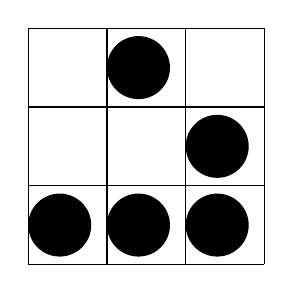
\begin{tikzpicture}
\draw [xshift=0.6cm,yshift=.5cm] (0,0) grid (3,3);
\fill
(1,1) \C
(2,1) \C
(2,3) \C
(3,2) \C
(3,1) \C;
\end{tikzpicture}
\newpage
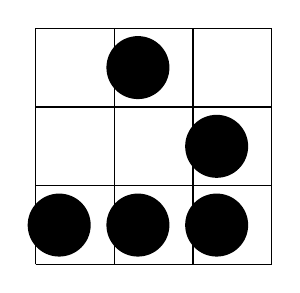
\begin{tikzpicture}
\draw [xshift=0.7cm,yshift=.5cm] (0,0) grid (3,3);
\fill
(1,1) \C
(2,1) \C
(2,3) \C
(3,2) \C
(3,1) \C;
\end{tikzpicture}
\newpage
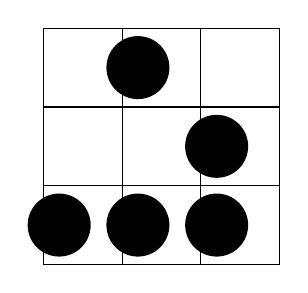
\begin{tikzpicture}
\draw [xshift=0.8cm,yshift=.5cm] (0,0) grid (3,3);
\fill
(1,1) \C
(2,1) \C
(2,3) \C
(3,2) \C
(3,1) \C;
\end{tikzpicture}
\newpage
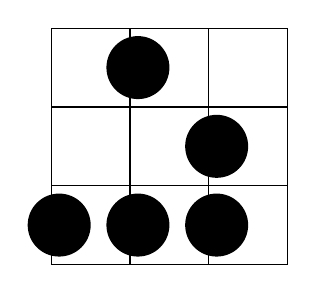
\begin{tikzpicture}
\draw [xshift=0.9cm,yshift=.5cm] (0,0) grid (3,3);
\fill
(1,1) \C
(2,1) \C
(2,3) \C
(3,2) \C
(3,1) \C;
\end{tikzpicture}
\newpage
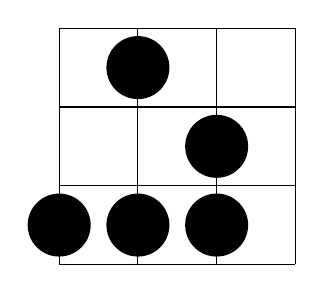
\begin{tikzpicture}
\draw [xshift=1.0cm,yshift=.5cm] (0,0) grid (3,3);
\fill
(1,1) \C
(2,1) \C
(2,3) \C
(3,2) \C
(3,1) \C;
\end{tikzpicture}
\newpage
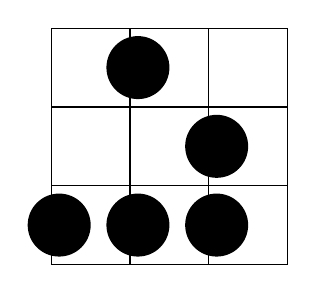
\begin{tikzpicture}
\draw [xshift=0.9cm,yshift=.5cm] (0,0) grid (3,3);
\fill
(1,1) \C
(2,1) \C
(2,3) \C
(3,2) \C
(3,1) \C;
\end{tikzpicture}
\newpage
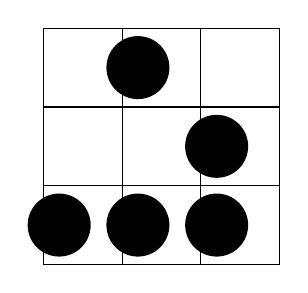
\begin{tikzpicture}
\draw [xshift=0.8cm,yshift=.5cm] (0,0) grid (3,3);
\fill
(1,1) \C
(2,1) \C
(2,3) \C
(3,2) \C
(3,1) \C;
\end{tikzpicture}
\newpage
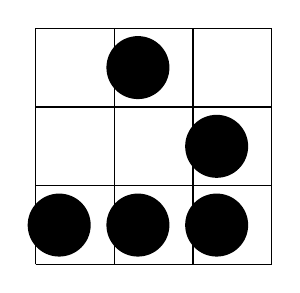
\begin{tikzpicture}
\draw [xshift=0.7cm,yshift=.5cm] (0,0) grid (3,3);
\fill
(1,1) \C
(2,1) \C
(2,3) \C
(3,2) \C
(3,1) \C;
\end{tikzpicture}
\newpage
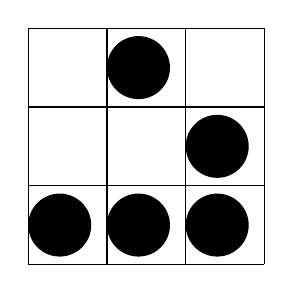
\begin{tikzpicture}
\draw [xshift=0.6cm,yshift=.5cm] (0,0) grid (3,3);
\fill
(1,1) \C
(2,1) \C
(2,3) \C
(3,2) \C
(3,1) \C;
\end{tikzpicture}
\newpage
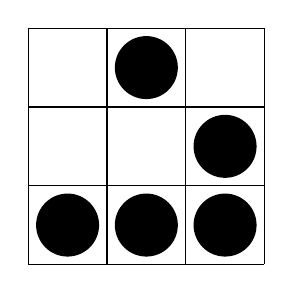
\begin{tikzpicture}
\draw [xshift=0.5cm,yshift=.5cm] (0,0) grid (3,3);
\fill
(1,1) \C
(2,1) \C
(2,3) \C
(3,2) \C
(3,1) \C;
\end{tikzpicture}
\newpage
\end{document}
